%In the introduction, we pointed out that the \ac{mhmm} assumption of the dwell times following geometric distribution is far from realistic in some applications. Hence, we proposed \ac{medhmm}, a novel approach that enables researchers to model a flexible range of state durations. The model incorporates dedicated dwell time distributions, which improves model interpretability and dwell time estimation \citep{Yu_2010}. However, the \ac{medhmm} comes at the expense of increased complexity, which leads to longer computation times and may require more resources (e.g. observations per subject). 
The purpose of the Monte Carlo simulation study was to compare the performance of the \ac{medhmm} and \ac{mhmm}. We simulated data from the Multilevel Explicit Duration Hidden Markov model using a full factorial design, varying three factors: 1) the number of hidden states, 2) the number of observations, and 3) the mean dwell time. Also, we included one extra simulation scenario to assess the effect of varying across-stats dwell times. We chose levels of each factor based on the \ac{mhmm} literature and summarized them in Table \ref{tb1}.\\ 

\begin{table}[h]

\caption{The summary of simulation study levels with three varying factors*}\label{tb1}
\begin{tabular}{c|c|c} 
\hline
Number of states ($m$)& Sample size ($N_{obs}$) & Mean dwell time ($d$) \\ 
\hline
3 & 200 & 1.4 \\
4 & 500 & 3.5 \\
 & 1000 & 19.5 \\
 & & 99.5 \\
\hline
3 & 500 & \{3.5, 19.5, 99.5\} \\
\hline
\end{tabular}
\flushleft
\footnotesize
\justifying
* The first four rows shows the simulation scenario levels to which we applied the full\\factorial design.
The last row includes the specifications of the additional simulation\\ scenario with varying across states dwell time. 
\end{table}

\subsection{Levels of the simulation study}
\subsubsection*{Number of states}
In order to assess how the number of parameters to infer influences the bias in its estimates, we considered two levels for a total number of states ${m \in \{3,4\}}$. With each level, the number of parameters increases quadratically with the number of states, i.e., the total number of parameters to estimate for both models is $m^2(N+1)$, where N is the number of individuals. The choices were made based on literature, which revealed that \ac{mhmm}s were typically fitted to three hidden states in \cite{maruotti_multilevel_2022}, \cite{Long_Tang_Wang_Jiang_2019}, \cite{de_haan_rietdijk_use_2017} and \cite{shirley_hidden_2010} and usually, not more than four hidden states \citep[see][]{Schafer_Wikle_VonBank_Ballard_Weegman_2020,inaba_mixed_2017}. 
%The two-state model was not considered in this simulation study due to its specific character in light of MEDHMM (the probabilities to transmit to any other state is fixed to 1 and the switches between states are purely dictated by the dwell time of a given state. 
\subsubsection*{Sample Size}
Based on the \ac{mhmm} literature, we decided to fix the number of individuals to ${N_{ind}=80}$, which indicated a median number of participants in studies that utilised \ac{ild} \citep[][]{altman_mixed_2007,Schliehe_Diecks_Kappeler_Langrock_2012,Schafer_Wikle_VonBank_Ballard_Weegman_2020, de_haan_rietdijk_use_2017,inaba_mixed_2017}. The levels of observations we set to ${N_{obs}\in \{200, 500, 1000\}}$. The literature included time series sample sizes ranging from $24$ in \cite{altman_mixed_2007} to $7257$ in \cite{inaba_mixed_2017}. However, we perceived the $24$ observations as not enough in the spirit of modern \ac{ild} designs and set the lower bound to $200$. The upper bound we chose to be ${N_{obs}=1000}$ since in behavioural settings this amount of observations per individual is seen as large.
\subsubsection*{Mean dwell time}
Since we based the design of the simulation study on the MHMM literature, we translated the information encoded in the self-transition probabilities of the TPM of MHMM into the expected dwell times that further were transformed to log-means and log-variances of the log-normal dwell time distribution (refer to next section for the details of transformation). The self-transition probabilities according to the reviewed literature including \cite{altman_mixed_2007,Schliehe_Diecks_Kappeler_Langrock_2012, de_haan_rietdijk_use_2017,Raffa_Dubin_2015,inaba_mixed_2017}, and \cite{Schafer_Wikle_VonBank_Ballard_Weegman_2020} were generally in range $\gamma_{ii}\in\{0.5-0.95\}$. We considered four levels of self-transition probabilities ${\gamma_{ii} \in \{0.5, 0.75, 0.95, 0.99\}}$, which correspondingly can be interpreted as low, medium, and high and very high state persistence and the mean dwell times that follow from them are ${d\in \{1.4,3.5,19.5,99.5\}}$. Note that the listed $d$ expected state durations were used in the full factorial design, where they were constant across states. The additional scenario involved ${d_a\in \{3.5,19.5,99.5\}}$ where each $d_a$ represented a different state-specific mean duration. 

% \begin{table}
% \tbl{Example of a table showing that its caption is as wide as
% the table itself and justified.}
% {\begin{tabular}{lcccccc} \toprule
% & \multicolumn{2}{l}{Conditions} \\ \cmidrule{2-4}
% Paper & States & Subjects & Occasions\\ \midrule
% \citep{maruotti_multilevel_2022}& 3 & 474 & 10 \\
% \citep{altman_mixed_2007}& - & 30 & 1-24 \\
% \citep{shirley_hidden_2010}& 3 & 240 & 168 \\
% \citep{de_haan_rietdijk_use_2017} &3 & 149 & 539 \\
% \citep{de_haan_rietdijk_use_2017} & 2 & 224 & 56 \\
% \citep{inaba_mixed_2017} & 2 & 89 & 20 \\
% \citep{Schliehe_Diecks_Kappeler_Langrock_2012} & 2 & 59 & 26\\
% \citep{Schafer_Wikle_VonBank_Ballard_Weegman_2020} & 4 & 50-100 & 5 \\
% \citep{Long_Tang_Wang_Jiang_2019} & 3 & 133 & 1064 \\
% \citep{inaba_mixed_2017} & 4 & - & 7257 \\ \bottomrule
% \end{tabular}}
% \label{Multilevel Hidden Markov models studies}
% \end{table}


\subsection{Data generation mechanism }
We simulated $128$ datasets from each of the $24$ scenarios using the factorial design on the parameters listed in Table \ref{tb1}. One additional scenario has been included to inspect the performance of the three-state model with varying between states dwell times. To ensure the stability of results and prevent convergence failures such as label switching, data were generated with two univariate normally distributed dependent variables with group-level means ${\bar{\mu}_{1i},\bar{\mu}_{2i}\in \{10-98\}}$ and variances ${\sigma_{1i}^2 \in \{20-150\}}$ for the first variable and ${\sigma_{2i}^2 \in \{25-187.5\}}$ for the second one (see Figure \ref{em_ds} in Appendix A for more details). In general, the parameters of emission distributions have been chosen such that the overlap proportion between subsequent state-dependent distributions was equal to $0.10$ for the first and $0.14-0.15$ for the second dependent variable. Random effects $u_{ni}$ were normally distributed with mean $0$ and variance ${\sigma^2_{[\mu]1i},\sigma^2_{[\mu]2i}=9}$ for both variables.

The dwell time probability was log-normally distributed (see Figure \ref{log_ds} in Appendix A for an illustration of the assumed distribution). The expected dwell times (medians of log-normal distributions) were set to ${d\in \{1.4,3.5,19.5,99.5\}}$ and obtained via transforming the self-transition probabilities ${\gamma_{ii} \in \{0.5, 0.75, 0.95, 0.99\}}$ using the formula\footnote{The expected state duration when the exponential distribution is assumed to be an approximation of the geometrical dwell time distribution for \ac{mhmm}.}: ${d=1/-\log(\gamma_{ii})}$. In order to get the log-mean and log-variance of the target distribution, we calculated ${\bar{\mu}_{[d]i}}$ by taking the logarithm of the expected dwell times $log(d)$. The log-variance ${\bar{\sigma}^2_{[d]i}}$ has been set such that the standard deviation of each dwell time distribution was equal to a third of the $d$ for, ${d\in \{1.4,3.5,19.5\}}$ except from when $d=99.5$ for which the standard deviation was a quarter of the value. In the result, the log-variances were equal ${\sigma^2_{[d\in \{1.4,3.5,19.5\}]i}}=0.096$ and ${\sigma^2_{[d=99.5]i}}=0.057$. The random effects $q_{[d]ni}$ were normally distributed, with mean $0$ and variance $\sigma^{2}_{[\bar{d}]i}=0.2$ that was common to all $d$. 

The TPM parameters were derived from multinomial logits where the off-diagonal entries were set so that there is an equal chance of transitioning to another state (e.g., the first row of TPM for $m=3$ was $\gamma_{1j}=[0 \,\,\, 0.5 \,\,\, 0.5]$). The individual-random effects of the transition distribution were normally
distributed with mean $0$ and variance ranging ${\sigma^2_{[\alpha]nij}=0.17}$ on the logit scale,
which translates to standard deviations on the off-diagonal entries in TPM ${\sigma_{\gamma_{nij}}=0.1}$, for ${i\neq j}$ on the probability scale. For simplicity, we will call the set of multinomial logits, the gamma distribution and the set of transformed logits representing the transition probabilities the transition distribution. The simulation script can be accessed via the link in the Supplementary Materials. 

\subsection{Model fitting}
Simulating data and fitting models was done in the statistical software R (R Core Team, 2022) and executed with the use of the Dutch National Supercomputer Snellius. We used developer versions of the \emph{mHMMbayes} package\footnote{The GitHub repository containing the \emph{mHMMbayes} package source code used in this analysis can be found under the following link: \url{https://github.com/emmekeaarts/mHMMbayes/tree/continuous-emiss}} \citep{mHMMbayespackage} and developer version of the \emph{medHMM} package\footnote{The GitHub repository containing the \emph{medHMM} package source code used in this analysis can be found under the following link: \url{https://github.com/emmekeaarts/medHMM/tree/dev}}, tailored accordingly to \ac{mhmm}s and \ac{medhmm}s for continuous dependent variables. Packages employ Bayesian estimation methods \citep{Emm_Th,Scott_2002} and forward-backwards algorithms to infer parameters \citep{Scott_2002}. 

As for, the \ac{mhmm} the (forward) probabilities of each state at every time point are calculated given the observed data. The hidden state sequence is then sampled from their full conditional posteriors in a backward pass given the (current) parameters of the model\footnote{For a detailed description of the estimation algorithm, see: \url{https://cran.rproject.org/web/packages\\/mHMMbayes/vignettes/estimation-mhmm.pdf}}. Based on the sampled hidden state sequence, the parameter estimates are updated by sampling them from their full conditional posteriors using either a Gibbs or a Random Walk Metropolis-Hastings step. In the case of \ac{medhmm}, the forward probabilities are calculated for each state and each duration $d$ in set $d\in[1,2,..,d_{max}]$. Then, the hidden states and their discrete durations are drawn from their full conditional posteriors in a backward pass, forming the hidden state sequence, and the rest follows. In this study, the $d_{max}$ was chosen such that it covered at least $95\%$ of the state persistence on different simulation levels (low, medium, high and very high) and is in the range $d_{max}\in\{100-600\}$. Besides that, the Bayesian approach to parameter estimation enables flexible parameter inference while avoiding the direct computation of complex likelihoods \citep{Frühwirth-Schnatter_2001,Scott_2002}. The approach has been shown to outperform other non-Bayesian methods in terms of computing speed \citep{Rydén_2008} and provides direct estimates for the fixed and random effects in the multilevel model. Furthermore, valuable by-products are produced in the inference process such as posterior standard deviations, credible intervals, or local decoding, which identifies the most probable state out of a series of discrete hidden states at each time point. 

We used $4000$ MCMC iterations to train both \ac{mhmm} and \ac{medhmm} and dropped the first $2000$ (burn-in) to reduce the influence of the starting values on the model convergence \citep{plummer2006coda}.
For emission and dwell time distributions, we used only uninformative and weakly informative hyper-priors that can be found in Table \ref{Ap_emiss_hp} and Table \ref{Ap_dwell_hp} in Appendix A. We used provided by software default hyper-priors for transition distribution that were uninformative and can be found in vignette of the \emph{mHMMbayes} \linebreak (Footnote 4, p. 11). In order to check the convergence, we fitted 5 randomly chosen out of 128 simulated datasets to both \ac{mhmm} and \ac{medhmm} with two additional chains specified with randomized starting values. The convergence of the group-level parameters (fixed effects) was assessed with the multivariate potential scale reduction factor \citep{Brooks_Gelman_1998} with a cut-off of ${\text{R} < 1.2}$ and inspecting trace plots of the parameters visually.

We inspected the group-level parameters of the emission, transition, and dwell time distributions with bias, precision, and coverage. Medians of the Bayesian posterior distributions of group-level parameters were used as point estimates. The differences between posterior medians and assumed true values were used as bias indicators. Relative percentage bias was reported to evaluate the size of the bias due to undercoverage with respect to the true unknown parameter to estimate. The relative bias of $5\%$ or less was considered acceptable. Additionally, the MHMM transition probability matrix (TPM) parameters were reported in two ways: 1) the direct TPM estimates from the MHMM algorithm, and 2) adjusted TPM such that the diagonal entries were set to 0. Since the true TPM probabilities were always balanced (the probability to switch to a different state was equal), the average across TMP entries absolute relative bias was reported. We also compared the expected dwell times for the MEDHMM (medians of the log-normal distribution) and MHMM (expected duration based on the self-transitions probabilities calculated using formula $1/-log(\gamma_{ii})$) and reported the average absolute bias for them. Note that average absolute bias measures were only reported for full the factorial simulation, excluding the additional scenario. 

The empirical standard errors were calculated and reported as the precision measure. The $95\%$ central credible intervals were computed as indications of the uncertainty about the parameters \citep{Lynch_2007}. Moreover, the coverage of estimates was assessed by the ratio of times the $95\%$ central credible intervals of model estimates overlap their true values. Coverage of $92\%$ and above was considered acceptable. The average proportion of hidden states correctly assigned by the local decoding \citep{Scott_2002}, as well as the average proportion of instances in which the decoding probability of the true state was at least $0.2$, were used to assess model performance for individual-level inference. The $\kappa$ statistic was used to control for the expected classification accuracy due to random chance \citep{Cohen_1960}.
The full reproducible code for the analysis is available in Supplementary Materials.

\subsection{Results}
In this section, we present the results of our simulation study, which aimed to compare the performances of MHMM and the newly introduced MEDHMM. The simulated data has been developed based on behavioural research conducted on continuous, intensive longitudinal data (mentioned in Section 3.1). We start with reporting the convergence performance for both models. Then, we describe the result for group-level estimates of emission distribution, transition probabilities and dwell time distribution parameters. Lastly, we report the state decoding performance, including empirically defined dwell times and the number of state switches. The additional scenario with varying dwell times was discussed in Section 3.4.6. All results\footnote{Two simulation scenarios for four-state MEDHMM (i.e., $d=3.5$ \& $500$ observations scenario and $d=99.5$ \& $1000$ observations scenario) were not included in the current manuscript because due to unstable Snellius infrastructure and reoccurring maintenance during last two weeks before submission, the MEDHMM scenarios did not manage to run. The results for the missing scenarios will be included as soon as the Snellius infrastructure will resume. The updated version of the manuscript will be uploaded to the research repository linked in Supplementary Materials.} are available for detailed inspection in Table \ref{tgr2_1}-\ref{mixed_sim} in Appendix D, and the most important results were described in the text below. 

\subsubsection{Convergence}
Overall, parameter convergence was achieved for group-level parameters in $100\%$ of MHMM assessed scenarios with the average potential scale reduction parameter $R \in \{1-1.1\}$. In MEDHMM the convergence was reached in $100\%$ of assessed three-states scenarios with $R=1$ for all group-level parameters. The major convergence issues occurred for MEDHMM in four-state scenarios assuming short dwell times ($d=1.4$ and $d=3.5$) for which only $87.5\%$ scenarios reached convergence. We would like to point out that in any case, all five considered MEDHMMs resulted in failure to converge. The model fitting didn't encounter any issues except 3 out of 128 simulated datasets in 2 scenarios fitted to MEDHMM which resulted in model execution failure due to overflow/underflow issues. The difference in available results was minimal and should not impact the Monte Carlo standard error. Hence, the MAP results were reported based on 125 simulated datasets for the explained 2 scenarios and on 128 simulated scenarios for the rest.  All trace plots can be found under the link listed in Supplementary Materials.


\subsubsection{Emission distributions}
%Bias The bias, precision, and coverage results were comparable in their magnitudes for both dependent variables. 
\emph{Bias}     In general, the MHMM performed better in recovering the means of the emission distributions in scenarios with shorter state durations (i.e., $d=1.4$ and $d=3.5$). The estimates of the means in MEDHMM were unsatisfactory for the $d=1.4$ scenarios and became closer to the truth as the assumed dwell time started increasing. Figure \ref{mubias} shows the relative bias (\% bias) of emission distribution means for two models and different simulation scenarios. For the shortest state duration scenarios, the MEDHMM overestimated smaller values and underestimated larger emission mean values, which resulted in \% bias ranging from $-43.7\%$ to $229.6\%$ in d=1.4 and from $-8.3\%$ to $30.7\%$ in d=3.5 for two dependent variables combined. The MHMM mean estimates were overestimated for the shorter dwell times, however, the bias values were between $-0.33\%$ and $1.74\%$. The relative bias in the emission distribution means was smaller than $5\%$ in $60\%$ cases for the MEDHMM and in $100\%$ for the MHMM. In addition, relative bias was less than $5\%$ for $100\%$ of means parameters for $d=19.5$ and $d=99.5$ for both models independently of the state number assumed and the observation length.
Variance components of the emission distribution were overestimated by both models. Larger deviations from the truth were present for MEDHMM in shorter dwell time scenarios, with bias from $214.6\%$-$2414.1\%$ when $d=1.4$ and from $19.3\%$-$318.9\%$ when $d=3.5$. The range of MEDHMM bias in variance estimates decreased noticeably for longer duration scenarios and ranged from $10.8\%$ to $37.4\%$ when d=$19.5$ and between $8.5\%$ and $37.6\%$ when $d=99.5$. The MHMM bias results for the variances ranged from $10.6\%$-$40.0\%$ and were stable across varying simulation scenarios. 

\emph{Precision}  The empirical standard deviation (ESE) of the all-group level parameters for MEDHMM was highly varying across observation length and state scenarios, especially for shorter dwell times (see Figure \ref{prec_emiss} in Appendix B). For MEDHMM within longer dwell time scenarios, the ESE values were similar across parameters and comparable to the ESE values for MHMM. For MHMM, the ESE for emission distribution group-level parameters were less prone to changes with varying simulation conditions and were between $0.55$ and $0.98$ for emission means and between $1.54$ and
$10.01$ for emission variances, while for the MEDHMM those ranges were, accordingly ${0.5-2.6}$, and ${1.6- 51.3}$. On average, the ESE values for the parameters were larger for the shorter observation lengths and smaller for the longer series lengths. 

\emph{Coverage}  The coverage of the group-level means is presented in Figure \ref{emiss_mu_cov} in the Appendix and indicates that the coverage of the parameters was above $92\%$ for $100\%$ of instances for MHMM and only above $92\%$ for MEDHMM in $53\%$ of instances. However, for longer dwell time scenarios, the coverage was acceptable in $100\%$ of the mean parameters when the dwell time assumed was $d=99.5$. The coverage for the variance component was poor, with a maximum value of $35.2\%$ for MEDHMM and $10.94\%$ for MHMM.  

\begin{figure}
\caption{\\Emission distribution means: \% Bias}
    \centering
    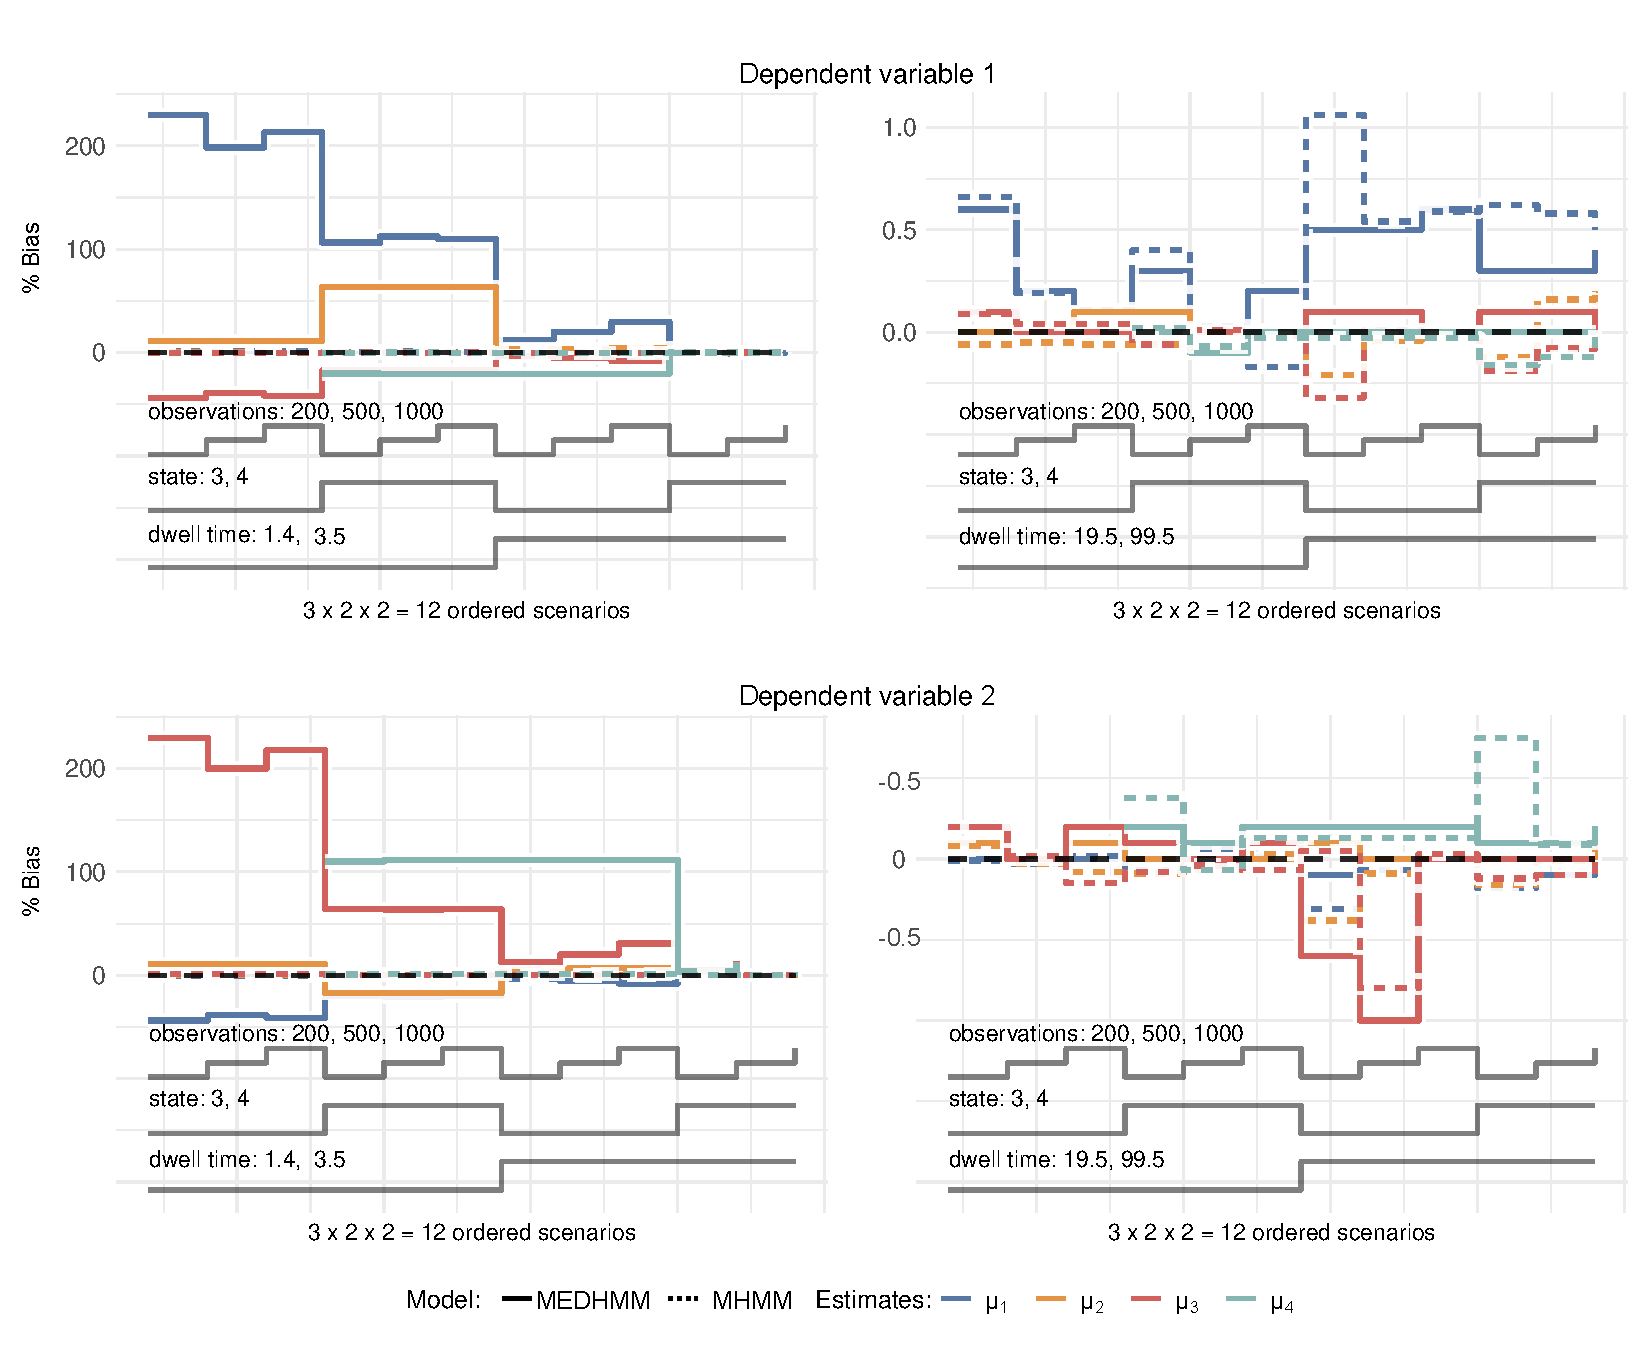
\includegraphics[width=\textwidth]{graphics/emiss_dep_bias2.pdf}
    \flushleft
    \footnotesize
    \justifying
    Plots illustrate the relative bias (\% Bias) of each emission distribution mean for every simulation scenario (note that the additional scenario with varying dwell time is omitted). The plots for each of the dependent variables are split onto two plots representing (from left) short state durations and longer state durations with dwell time $d\in \{1.4, 3.5\}$ for the left plot and $d\in \{19.5, 99.5\}$ for the right plot. Each colour represents the state-specific emission mean parameters, and line type is the model indicator.
    \label{mubias}
\end{figure}



\subsubsection{Transition distribution}
Overall, the performance of MEDHMM for the group-level transition distribution parameters worked better in terms of bias and coverage of the true parameters in comparison to the MHMM. \\
\emph{Bias}     The MEDHMM bias in TPM parameter estimates was below $5\%$ in $66\%$ of scenarios. The bias values for MEDHMM were influenced by the number of observations, states and dwell time assumed. The model had noticeably worse performance in bias for the scenarios with $d=1.4$ and $d=3.5$ when four states were assumed, irrespectively of the observation length (see Table \ref{tgr2_1}-\ref{tgr1_4} in Appendix D for detailed values). For three-state scenarios, MEDHMM bias was larger than $5\%$ of the true value only when $d=1.4$. For the HMMM's untransformed TPM, all group-level self-transition probabilities were consistently overestimated and resulted in the relative bias between $-39.54\%$ and $-0.59\%$. More significant bias values were recorded for $d=1.4$ scenarios and $d=99.5$. \newpage Since all group-level TPM parameters in MHMM are estimated as a system, the probabilities of transitions between two different states were systematically underestimated for the method. Only $10\%$ of parameters estimated by MHMM had relative bias smaller than $5\%$.

\emph{Precision}    In terms of precision, the values of ESE for the MEDHMM were more generous in comparison to the MHMM and ranged from $0.01$-$0.2$ while for the MHMM the ESE were between $0.01$ and $0.04$. In general, the ESE estimates were marginally decreasing with the number of observations.

\emph{Coverage}     The coverage for the MHMM untransformed TPM parameters was not satisfactory and did not exceed $70\%$ for any parameter. The coverage for the MEDHMM TPM parameters was acceptable in $57\%$ of its estimates. 

Figure \ref{trans_bias} illustrates the comparison of the transformed MHMM TPM (without the diagonal entries) and the MEDHMM in terms of absolute bias. The results showed, that although the untransformed parameters of MHMM were not representing the truth as good as the MEDHMM, the model was able to recover the information about equal chance of switching to any state assumed by the simulation study. Especially when the $m=4$ and $d=1.4$ the values of the transition probabilities were nearer to the true values in comparison to the MEDHMM. For the scenarios with the dwell time assumed to be greater than $d=3.5$ the transition probabilities were better recovered by the MEDHMM when compared to the transformed MHMM TPM. 

\begin{figure}[h]
\caption{\\The average absolute relative bias in adjusted transition distribution}
    \centering
    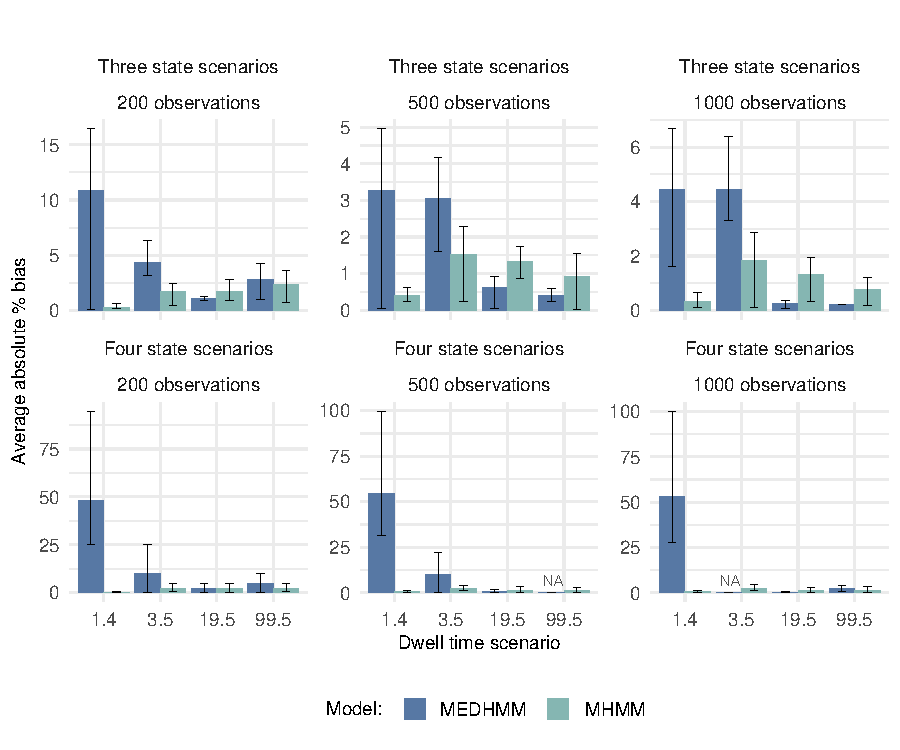
\includegraphics[width=0.8\textwidth]{graphics/transition_prob_biasv2.pdf}
    \flushleft
\footnotesize
\justifying
The bar plots represent the averaged over transition probabilities for the MHMM adjusted transition probabilities \% bias for each scenario (i.e. for the three-state scenario in MEDHMM we took the absolute \% bias of non-zero transition probability matrix (TPM) entries and calculated the mean of those values; for MHMM we adjusted the TPM such that the diagonal entries (self-transitions) were fixed to 0 and then proceeded as with the MEDHMM's TPM). The error bars represent the range of the absolute \% bias for the transition probability values within a given scenario and model. Each panel is the same state and observation scenario where the first row is the three-state scenario and the second plot is the four-state scenario. The y-axis indicates the dwell time scenario, and colours represent different models. 
    \label{trans_bias}
\end{figure}


\subsubsection{Dwell time distributions}
Note that the parameters of log-normal dwell time distribution were estimated and reported only by the MEDHMM. 

\emph{Bias}     Overall, the performance in bias for the log-means of the dwell time distribution improved with increasing assumed dwell times. The bias estimates did not depend on the varying number of states. The log-mean values were overestimated majorly for $d=1.4$ with bias equal form $324\%-686\%$ of the true value. The number of observations tended to reduce the absolute bias, but did not improve the estimates when $d=1.4$. Two scenarios with an observation length of $200$ and $d=99.5$ assumed were slightly underestimated, however, still did not exceed the cut-off value of acceptable bias. The relative bias for log-mean estimates was lower than $5\%$ in $47\%$ of scenarios. In terms of log-variances, the absolute bias estimates for MEDHMM were least significant for the scenarios with $d=19.5$. The model tend to overestimate the log-variances in general, and the bias was decreasing with the length of the observation sequence. The tendencies in the estimates were not dependent on the number of states estimated. Values of \% bias ranged from $-100\%$ to $142.9\%$. The bias was less than $5\%$ of the true value for $41\%$ of the log-variance parameters. The best results for log-variances were obtained for simulation scenarios with dwell times $d\in\{99.5, 19.5\}$ independently of the state and observations scenarios.

\emph{Precision}    Precision estimates (ESE) for the log-means were less than $0.001$ on the log scale and were ranging from $0.001$ to $0.6$ on the log scale for the log-variance components.

\emph{Coverage}     The coverage for the log-mean parameters reached an acceptable level of $92\%$ in $33\%$ of scenarios and was within the satisfactory range for scenarios with d=$19.5$ and d=$99.5$. The number of states and observations had no impact on the coverage scores for the parameters. Moreover, the coverage for the log-variance estimates was slightly better, since $46\%$ of the total cases had coverage above the acceptable threshold. The coverage rates of the log-variance were increasing with the assumed dwell time value, hence they were most satisfactory for $d=19.5$ and $d=99.5$ and no influence of the varying observation sequence or the number of states was recorded. 

In order to relate the MEDHMM dwell time estimates to MHMM the average absolute relative bias was calculated and shown in Figure \ref{exp_dwell_bias}. Note that we treated the median of the log-normal distribution and the expected value of the exponential distribution as the expected dwell time for the MEDHMM and MHMM accordingly. The comparison revealed that according to the average absolute bias, the MEDHMM expected state duration was further from the assumed truth for all scenarios with $d=1.4$. The average absolute relative bias within MEDHMM estimates tended to decrease with longer durations. On the other hand, the statistics calculated for the MHMM dwell time estimates became greater with longer dwell time scenarios and the values were more prominent for more complex four-state scenarios. 
\begin{figure}[h]
\caption{\\The average absolute relative bias for the expected dwell times } 
    \centering
    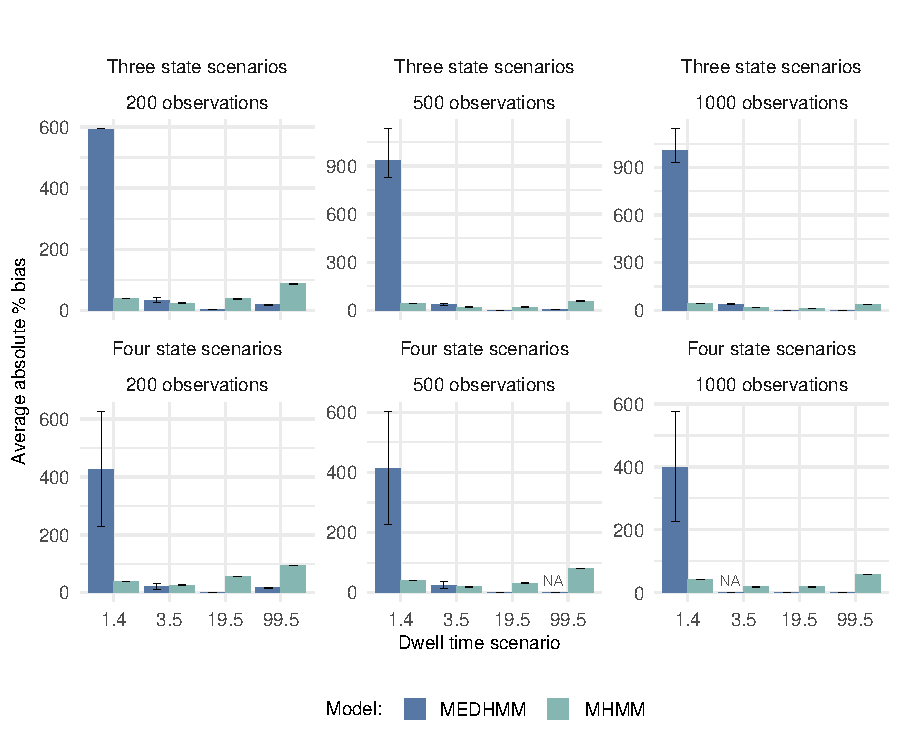
\includegraphics[width=0.8\textwidth]{graphics/expected_dwell_biasv2.pdf}
\flushleft
\footnotesize
\justifying
The bar plots represent the averaged over the state-specific expected dwell times \% bias for each scenario (i.e. for the three-state scenario in MEDHMM we took the absolute \% bias of the expected state durations for state 1, 2, and 3 and calculated the mean of those three values). The error bars represent the range of the absolute \% bias for the state-specific values within a given scenario and model. Each panel is the same state and observation scenario where the first row is the three-state scenario and the second plot is the four-state scenario. The y-axis indicates the dwell time scenario, and colours represent different models. 
\label{exp_dwell_bias}
\end{figure}

\subsubsection{State decoding derived measures}
The subject-specific state decoding was inspected in three ways: the proportion of states correctly decoded for each scenario visualized in Figure \ref{decoding_kappa}; the average number of switches in state decoding sequences in Figure \ref{state_switches} in Appendix B; and the average empirical duration of each state within given scenarios showed in Figure \ref{empiric_dwell} in Appendix B. In terms of decoding accuracy, the MHMM states were recovered in $99\%$ of scenarios. On the contrary, the MEDHMM recovered $81\%$ of the states' position. The state decoding for the MEDHMM failed for the shortest dwell times assumed. The MEDHMM did significantly worse for scenarios with a shorter duration of $d=1.4$ and $d=3.5$. However, for scenarios with dwell time $d=19.5$ and $d=99.5$ the Kappa statistic was greater for the MEDHMM when compared to the MHMM, but the differences were not larger than the $0.1\%$ change. The average number of switches for each scenario was recovered almost perfectly for the MHMM. The MEDHMM underestimated the average number of switches for the scenarios with $d=1.4$ and $d=3.5$. The estimated number of switches in MEDHMM tended to be closer to the switches count in simulated data with the increasing sequence length and number of states, especially for the $d=3.5$ scenario. In terms of the estimation of the state persistence according to the local decoding, the MHMM empirical dwell times were closer to in-sample dwell times for all simulation scenarios. The MEDHMM decoding showed overestimated state persistence when the shorter dwell time was assumed and was closest to the in-sample state duration for the scenario with the longest dwell time assumed d=99.5. 

\subsubsection{Additional Simulation scenario: Dwell time varying between hidden states}
 In general, the MEDHMM was able to recover varying dwell times across states. Log-means and log-variances were generally estimated within the satisfactory thresholds for bias and coverage, except for the log-means for the state with the shortest persistence, for which the value was slightly overestimated. The empirical standard deviations were smaller than $0.1$. The comparison of the expected state persistence showed that the MEDHMM was able to recover the expected durations, the MHMM underestimated the expected dwell time values and had difficulty estimating longer dwell times (see Table \ref{mix_table_exp_dwell}). Regarding the TPM parameter estimation, the MEDHMM did well in terms of bias and coverage with minor instabilities for two out of six parameters. On the other hand, the MHMM TPM estimates were not satisfactory, with only one probability recovered with satisfactory $\%bias$. In terms of the emission distribution means, the estimates derived by MEDHMM and MHMM were similar and had almost identical ESE. The Bias and coverage values for the mean parameters were acceptable for MHMM and mostly acceptable for MEDHMM (the first state means resulted in  $79.7\%$ coverage value). The variance components of the emission distribution were consistently overestimated by two models, and none of them reached acceptable coverage or bias. The ESE of the variances were larger for the MEDHMM and ranged from $1.4$-$12.4$ while for the MHMM they were between $1.8$ and $10.4$. In MHMM the self-transition probabilities were slightly underestimated however the self-transitions probabilities for the states with duration assumed to be $d=19.5$ and $d=99.5$ were close to the assumed proportions and only for these two TPM entries bias was less than 5\% of their expected true value. The TPM parameters for the MHMM had on average larger ESE when compared to MEDHMM and none of its parameters had satisfactory coverage. Regarding state decoding, the Kappa statistics were $99.7\%$ for the MEDHMM
and $99.9\%$ for MHMM. The average number of switches in-sample was $11$ and was recovered correctly by the MEDHMM while the MHMM average count of switches was $12$. The empirical dwell times derived from the local decoding mostly agreed with the in-sample estimates.  
All MAP estimates for the group-level parameters were summarised and are available for detailed inspection in Table \ref{mixed_sim} in Appendix D.

\begin{table}
\caption{The expected dwell times for the MEDHMM \& MHMM for varying between states dwell time scenario}
\centering
\begin{tabular}{cccccc} 
\toprule
 &  & \multicolumn{2}{c}{MEDHMM} & \multicolumn{2}{c}{MHMM} \\ 
\cmidrule{1-2}\cmidrule(lr){3-4}\cmidrule(lr){5-6}
State & Expected Dwell time & Median (ESE) & \% Bias & Median (ESE) & \% Bias \\ 
\midrule
1 & 3.5 & 3.94 (0.05) & 12.86 & 2.36 (0.16) & -32.08 \\
2 & 19.5 & 19.30 (0.06) & -0.67& 12.67 (1.14) & -34.99 \\
3 & 99.5 & 97.51 (0.05) & -2.21 & 69.30 (6.89) & -30.35 \\
\bottomrule
\label{mix_table_exp_dwell}
\end{tabular}
\end{table}


\begin{figure}[h]
\caption{\\The decoding accuracy (Kappa statistics) of all simulation scenarios and both models}
    \centering
    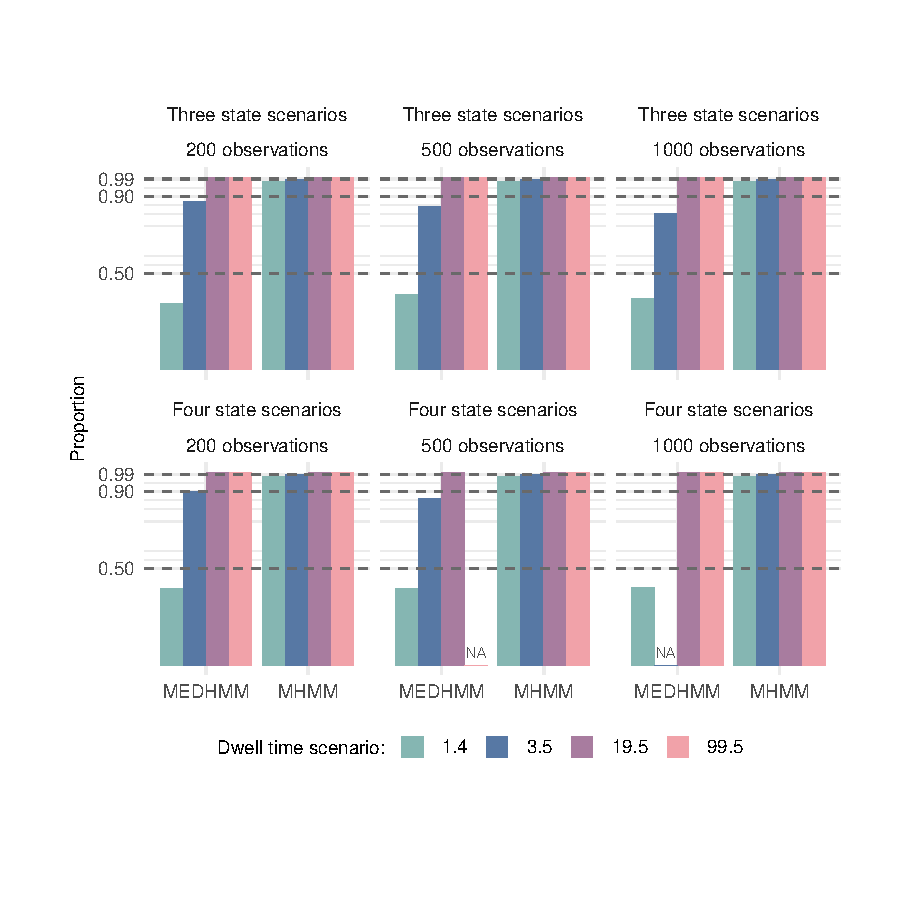
\includegraphics[width=0.8\textwidth]{graphics/state_decoding_simulation.pdf}
    \flushleft
    \footnotesize
    \justifying
    The bar plots show how Kappa statistics compare across varying simulation scenarios and models. Each panel is the same state and observation scenario where the first row is the three-state scenario and the second plot is the four-state scenario. The y-axis represents the models for which the statistics are calculated, and the colour is an indicator of the dwell time scenario.   
    \label{decoding_kappa}
\end{figure}